\chapter{Model Predictive Control of AToD}\label{ch:mpc}
\section{Linear-Discrete Time Model}\label{sec:linear_discrete_time_model}
The model derived in this section is partially inspired from \cite{zhang2016}. \\
Consider a transportation network be composed of $|\mathcal{V}|$ stations scattered around a space $\Omega$ and $|\mathcal{A}|$ multi-occupancy, goods-carrying vehicles working within the same space $\Omega$. Within this context, customers are assumed to requests rides only from the abovementioned stations. Similarly, goods can be carried out only from one station to another. With this assumption, stations and customers can be considered synonims within this section. \\
Similarly to the model described in \chapref{sec:vc_model}, other than carrying goods or people, vehicle are expected to \textit{(i)} serve clients from one station to another and \textit{(ii)} reach locations in $\Omega$ in order to avoid system imbalance. \\
Let $d_{ij} \in \mathcal{R}_{\ge0}$ be the total lenght of a road \(\langle i,j\rangle\). Let $v^a_{ij}(t) \in \{0,1\}$ indicate whether a transporting vehicle $a \in \mathcal{A}$ is moving from station $i$ to station $j$ ($v^a_{ij}(t) = 1$) and, likewise, $w^{a}_{ij}\in \{0,1\} $ whether an empty vehicle is moving from $i$ to $j$ ($w^{a}_{ij}(t)= 1$). Let $V_{ij}(t) = \sum_{a \in \mathcal{A}} v^{a}_{ij}(t) +w^{a}_{ij}(t)$ being the total number of vehicles currently circulating on the street $\langle i,j\rangle$, it follows that $V_{ij}(t) \in \mathbb{N}_+$. \\
When a vehicle is in transit, it is essential to monitor the anticipated duration until it reaches its destination. In order to do so, let's assume the road $\langle i,j\rangle$ to have a speed limit $l_{i,j}$. Accordingly, since the system is dealing with fully autonomous vehicles, in a typical driving scenario, one can safely assume this to be the cruising speed as well. In other words, one can assume the vehicles to be driving with a speed $l_{i,j}$ over $\langle i,j\rangle$ in normal road conditions.  Motivated by safety concerns, the cruising speed cannot be consistently maintained at \(l_{i,j}\) due to various factors. These factors may include road conditions, weather conditions, traffic density, or any unforeseen circumstances. Therefore, the actual cruising speed during the journey over road \(\langle i,j\rangle\) may vary based on these dynamic elements, ensuring that the autonomous vehicles can adapt to changing conditions and prioritize safety over a fixed cruising speed. One factor which is directly controllable is the traffic density. Therefore, taking inspiration from the BPR model (\figref{fig:bpr_models_approx}), we can approximate the cruising speed according to the amount of vehicles on the road. More specifically, we can modify \equaref{eq:model_bpr_approximation} to reflect this condition, and therfore rewriting it as \\
\begin{equation}
	\begin{aligned}	
		s_{ij}(V_{ij}) &= \begin{cases}
			l_{ij} \quad\quad &\text{if } V_{ij}\in[0,V_{ij}^{th}]\\ 
			l_{ij} - b\cdot(V_{ij} - V_{ij}^{th}) \quad\quad &\text{if }V_{ij}\in[V_{ij}^{th}, V_{ij}^{max}]\\ 
			0\quad\quad &\text{if }V_{ij} \ge V_{ij}^{max}\\ 
		\end{cases}\\
		\text{with } b  &=  \dfrac{l_{ij}}{ V_{ij}^{th} -  V_{ij}^{max}}
\end{aligned}
	\label{eq:model_bpr_approximation2}
\end{equation}
An example can be seen in \figref{fig:speed_model}. The last case, i.e. when $V_{ij} \ge V_{ij}^{max}$, is inspired from the congestion model used in \secref{sec:vc_model} and in this case is modeling stale mate traffic. Intuitively, if too many cars are on the road, these will not be able to circulate with a high speed and eventually stop-and-go traffic will be created. \\
From the definition, it follows that $s_{if}$ is defined as $s_{ij}: \mathbb{N}_{+} \rightarrow \mathbb{R}_{\ge 0}$.

\begin{figure}[t]
	\centering
	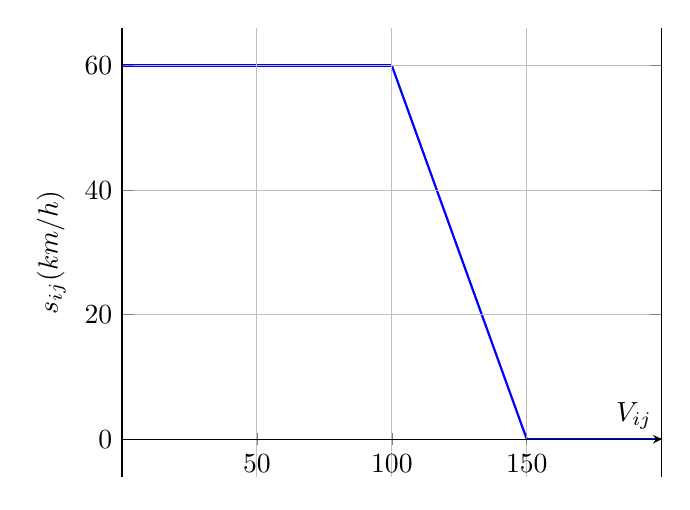
\begin{tikzpicture}
		\begin{axis}[
			xlabel={$V_{ij}$},
			ylabel={$s_{ij} (km/h)$},
			domain=0:250, % adjust the domain based on your preference
			samples=40,
			grid=both,
			axis x line=middle,
			%ymin=-1, % Set the minimum y-axis value
			%ymax=1.4, % Set the maximum y-axis value
			axis on top,
			legend pos=north east
			]
			% Piecewise function
			\addplot[blue, thick, domain=0:100] {60};
			\addplot[blue, thick, domain=100:150] {60 - 1.2*(x-100)};
			\addplot[blue, thick, domain=150:200] {0};
			%\addlegendentry{B}
		\end{axis}
	\end{tikzpicture}
	\caption[Cruising speed in function of traffic density]{Cruising speed in function of traffic density. In this example, $l_{ij} = 60 km/h,V_{ij}^{th} = 100$,$V_{ij}^{max} = 150$.  }
	\label{fig:speed_model}
\end{figure}
This allows to effectively track the position of the vehicle in terms of time as well. However, the position should be tracked only if the vehicle is currently driving on the street. 
Therefore, position of the vehicle $a$ over $\langle i,j\rangle$ is propagated using \equaref{eq:position_propagation}. 
\begin{equation}
	x^a_{ij}(t+\delta) =\begin{cases}
		 x^a_{ij}(t) + s_{ij}(V_{ij}(t))\cdot\delta & \text{if } v^a_{ij}(t) + w^a_{ij}(t)= 1 \\
		 
		 0& \text{if } v^a_{ij}(t) + w^a_{ij}(t)= 0\\
		 0& \text{if }i=j \\
		 %0 & \text{otherwise}
	\end{cases}
	 \label{eq:position_propagation}
\end{equation}
As mentioned above, \equaref{eq:position_propagation} tracks the position of a moving vehicle, i.e. takes care of the state of moving vehicles. In addition to this, the model also needs to track the number of vehicles currently stationed in $i$. This is achieved by introducing an additional variable $f^a_i(t)$, which indicates whether a vehicle arrived at a station $i$. It is defined as following.
\begin{equation}
	f^a_{i}(t) =\begin{cases}
		1 & \text{if }x^a_{ji}(t)= d_{ji}\\
		0 & \text{otherwise}
	\end{cases}
	\label{eq:station_propagation}
\end{equation}
This is propagated with the help of the indicator function. 
\begin{equation}
	f^a_i(t+1) =f^a_i(t) + 1_{d_{ji} = x^a_{ji}(t)} - \sum_{j\in\mathcal{V}}(v_{ij}^a + w_{ij}^a) %1_{d_{ji} \neq x^a_{ji}(t)}
	\label{eq:stationed_propagation_ind}
\end{equation}
\equaref{eq:stationed_propagation_ind} also ensures that a vehicle performs an action on the road $\langle i,j\rangle$ only when stationed at $i$.\\
%\begin{equation}
%	f^a_i(t+1) = f^a_i(t) +1_{d_{ji} = x^a_{ji}(t)} - \sum_{j \in \mathcal{N}}( v^a_{ij} + w^a_{ij})
%	\label{eq:stationed_propagation}
%\end{equation}
The function $1_x$ is commonly known as the indicator function, denoting a Boolean variable x that can take values {true, false}. Specifically, $1_x$ is defined as follows:
\begin{equation}
	1_x = \begin{cases}
		1 & \text{if } x \text{ is true} \\
		0 & \text{if } x \text{ is false}
	\end{cases}
\end{equation}
In other words, $1_x$ equals 1 when x is true and equals 0 when x is false, making it a convenient way to express the truth value of the variable x in mathematical notation.\\
Crucially, the vehicles can not perform the aforementioned actions, i.e. waiting, routing and rebalancing, at the same time and this must be insured. Furthermore, the vehicles can not perform the actions on multiple stations or roads. Therefore, the following constraint is necessary. \\
\begin{equation}
	\sum_{i \in \mathcal{V}}(f^a_{i}(t+1)+\sum_{j \in \mathcal{V}}v^a_{ij}(t) + \sum_{j \in \mathcal{V}}w^a_{ij}(t)) = 1\label{eq:no_3_actions}
\end{equation}
This also implies that, if a vehicle is stationed at a station $i$, it can not have a position anywhere else. 
\begin{equation}
	%0<\sum_{i \in \mathcal{V}}(f^a_{i}(t)+\sum_{j \in \mathcal{V}}\dfrac{x^a_{ij}(t)}{d_{ij}}) \leq1 \label{eq:position_station}
	%d_{ji}
	\sum_{i \in \mathcal{V}}(f^a_{i}(t)+1_{ x^a_{ji}(t)\neq 0}) =1 \label{eq:position_station}
\end{equation}
In other words, if I vehicle is travelling through an edge $\langle ji\rangle$, it can only be stationed at $i$ if it finished travelling. \\
While it is on the one hand interesting to know which station is currently hosting which vehicle, it is more important to know the amount of vehicles currently circulating in the system. This can be achieved by flipping the idea and therefore calculating how many vehicles out of the total number is currently not stationed. 
\begin{equation}
	F(t) = |\mathcal{A}| - \sum_{i \in\mathcal{N}}\sum_{a \in\mathcal{A}}f^a_{i}
\end{equation}
Furthermore, one can also calculate the required time $T_{ij}(t)$ based on the speed approximation, as shown in \equaref{eq:required_time}. 
\begin{equation}
	T_{ij}^a(t) = \begin{cases}
		\dfrac{d_{ij} - x^a_{ij}(t)}{s_{ij}(V_{ij}(t))} &\quad \text{if } x_{ij}^a(t) > 0\\
		&\\
		0 &\quad\text{otherwise }
	\end{cases}
	\label{eq:required_time} 
\end{equation}

Denoted by $p_{ij}(t)$ and $g_{ij}(t)$ are the transportation and goods delivery requests respectively starting from station $i$ and headed to $j$. Let $o^p_{ij}(t)$ and $o^g_{ij}(t)$ denoting the number of outstanding requests from $i$ to $j$ for people or goods, respectively, one can describe its propagation as follows:

\begin{equation}
	\begin{aligned}
		o^p_{ij}(t+1) =& o^p_{ij}(t) + p_{ij}(t) - \sum_{a \in \mathcal{A}} P_a\cdot v^a_{ij}(t)\\
			o^g_{ij}(t+1) =& o^g_{ij}(t) + g_{ij}(t) - \sum_{a \in \mathcal{A}} G_a \cdot v^a_{ij}(t)\\
	\end{aligned}
	\label{eq:demand_time}
\end{equation}
%Furthermore, when a vehicle leaves, it can only leave 
It follows then that vehicles can not transport more than what requested, i.e.:
\begin{equation}
	\begin{aligned}
	\sum_{a \in \mathcal{A}}  P_a\cdot v^a_{ij}(t) &\leq o^p_{ij}(t) + p_{ij}(t) \\
	\sum_{a \in \mathcal{A}} G_a \cdot v^a_{ij}(t) &\leq o^g_{ij}(t) + g_{ij}(t)
	\end{aligned}
	 \label{eq:no_more_than_request}
\end{equation}


At this point, the definition of the control and the state of the system is complete. More specifically, the state of the system is described by the number outstanding requests $o_{ij}(t)$, the position of each moving vehicle $x_{ij}(t)$ and the position of each idle vehicle $f^a_{i}(t)$. Let the vector x(t) be the column vector column vector created by reshaping and concatenating $o_{ij}(t)$, $x_{ij}(t)$, $T_{ij}^a(t)$ and $f^a_{i}(t)$, the set of feasible states $\mathcal{X}$ is defined as follows. 

\begin{equation}
	\mathcal{X} := \left\{
	\begin{aligned}
		& o^p_{ij} \in (\mathbb{N}_+)^{|\mathcal{V}|},o^p_{ii} = 0, o^g_{ij} \in (\mathbb{N}_+)^{|\mathcal{V}|},o^g_{ii} = 0   \\
		 x = [o^p_{ij},o^g_{ij}, x_{ij}^a, f^a_{i}, T_{ij}^a]^T \Bigg| &f^a_{i} \in \{0,1\}^{|\mathcal{A}||\mathcal{V}|}, \text{(\ref{eq:position_station})} \\
		&  x_{ij}^a\in (\mathbb{R}_{\ge 0})^{|\mathcal{A}||\mathcal{V}|}, T^a_{ij} \in (\mathbb{R}_{\ge 0})^{|\mathcal{V}|} \\
	\end{aligned}
	\right\}
\end{equation}
%Note that because of  \equaref{eq:position_propagation}, the set of feasible states is time-dependent. 
Similarly, considering the control inputs $v^{a}_{ij}(t)$ and $w^{a}_{ij}(t)$, one can derive the set of feasible control set $\mathcal{U}(t)$ as follows. 
\begin{equation}
	\mathcal{\mathcal{U}}(t) := \left\{
	\begin{aligned}
		&v^a_{ij} \in \{0,1\}^{|\mathcal{A}||\mathcal{V}|}, v^a_{ii} = 0 \\
		u = [v^{a}_{ij}, w^{a}_{ij}]^T \Bigg|&w^a_{ij} \in \{0,1\}^{|\mathcal{A}||\mathcal{V}|},w^a_{ii} = 0 \\ 
		&\text{(\ref{eq:no_3_actions}),(\ref{eq:no_more_than_request})
		} \\
	\end{aligned}
	\right\}
\end{equation}
Since (\ref{eq:no_3_actions})-(\ref{eq:no_more_than_request}) depend on time, $\mathcal{U}(t)$ is also time-dependent. \\
Thanks to these formulations, the system can be written as a linear time-dependent system of the form
\begin{equation}
	x(t+1) = Ax(t) + Bu(t)\label{eq:normal_system}
\end{equation}
where $x(t) \in \mathcal{X}$, $u(t) \in \mathcal{U}(t)$ and $A$ and $B$ are the matrix associated to the coefficients of (\ref{eq:position_propagation}), (\ref{eq:stationed_propagation_ind}) and (\ref{eq:demand_time}). \\


\subsection{Model Evaluation}
Some comments are in order. Requests are treated considering customers and goods as single entities. More specifically, if a group consisting of three customers reach a station, this is treated as three individual requests, therefore $p_{ij}(t) = 3$. While this simplifies the model description and reflects the requirements for goods delivery, it would create an inconvenient scenario for traveling customers. As a matter of fact, it is not hard to envision situations where a group of travelers would like to travel together. However, it is out of the scope of this work to treat this scenario. One might also argue that this simplification effectively treats the model as if vehicles where single-occupancy and it is true in terms of intuition, this addition allows to reduce the number of variables by a constant factor, i.e. the sum of all vehicles' capacity. \\
The system described in \equaref{eq:normal_system} implicitely assumes the customer arrival to be known a priori. In order words, this is not treated as noise, but rather as a known quantity. 
\begin{equation}
	x(t+1) = Ax(t) + Bu(t) + w(t)\label{eq:disturbed_mpc_formulation}
\end{equation}
where $x(t) \in \mathcal{X}$, $u(t) \in \mathcal{U}(t)$, $w(t) = [p_{ij}(t)\quad g_{ij}(t)\quad0\quad0 \quad0]^T$ and $A$ and $B$ are the matrix associated to the coefficients of (\ref{eq:position_propagation}), (\ref{eq:station_propagation}) and (\ref{eq:demand_time}). \\
\equaref{eq:disturbed_mpc_formulation} treats customer arrival as noise, or disturbance, which makes reasoning on the system considerably harder. Several techniques (\cite{Campo1987RobustMP}, \cite{LANGSON2004125}) have been proposed to deal with this type of MPC systems, i.e. Robust MPC.  Alternatively, some work propose solutions to estimate this quantity using Deep Learning techniques (\cite{9202791}, \cite{8569427}).
However, the analysis of those techniques and their performance in this scenario is out of the scope of this work.
Similarly to \secref{sec:vc_model}, the model must take into account that stations do not have unlimited amoun t of parking spots. As a consequence, the number of vehicles stationed must be limited accordingly and this is achieved as follows. 
\begin{equation}
	\sum_{a \in \mathcal{A}}f^a_i(t) \leq C_i
	\label{eq:parking_limit}
\end{equation}
where $C_i$ indicates the number of parking spots available at $i$. \\
This is a crucial 

\section{Problem Formulation}
The MPC for the AToD problem is formulated as follows. \\
Given $x(t) \in \mathcal{X}$, determine the controls $u(t), \dots, u(t+N)$ according to the following optimization problem.
\begin{equation}
	\begin{aligned}
		\underset{\substack{u(t), \dots, u(t+N)}}{\text{\textbf{min}}} \quad & J_f(x(N))+\sum_{t=0}^{N-1}I(x(t)) \\
		\text{\textbf{s.t.}} \quad & x(t+1) = Ax(t) + Bu(t)  \\
		& x(t) \in \mathcal{X}, \ u(t)\in \mathcal{U} \\
		%& k = t, \dots, t+N\\
		&x(N) \in \mathcal{X}_f\\
	\end{aligned}
	\label{eq:mpc_atod}
\end{equation}
where $J_f(x(t+N))$ is the terminal cost function and $\mathcal{X}_f$ is the terminal set. \\
As the main goal is to prove the stability of (\ref{eq:mpc_atod}), a proper definition of those will facilitate this objective. The strategy used to prove stability is the one described in \secref{sec:stable_mpc_systems}. For this purpose, the terminal set is required to be defined around an equilibrium point $x_*$. A good canidate for the equilibrium point in such systems can be found by observing that the system remains at a equilibrium whenever no more requests arrive and the are no more outstanding requests within the system. In other words, when 
\begin{align*}
	p_{ij}(t) &=0 \\
	g_{ij}(t) &=0\quad\quad \forall i,j\in\mathcal{V}\\
	o^p_{ij}(t) &=0\\
	o^g_{ij}(t) &=0\\
\end{align*}
By \equaref{eq:demand_time}, this implies that, eventually, no more vehicles will transport goods or people anymore. Furthermore, one can also conclude that vehicles will also stop rebalancing themselves. Therefore, $o_{ij}, x_{ij}^a$ and $T_{ij}^a$ all assume value zero. However, there is no way of knowing exactly where vehicles are going to be stationed. Upon inspection, however, one can canclude that vehicles must be stationed somewhere, since they are not driving. In other words, $f^a_{i}$ could assume any value in $\{0,1\}^{|\mathcal{A}||\mathcal{V}|} $ except $ \{0\}^{|\mathcal{A}||\mathcal{V}|}$. Furthermore, at equilibrium, all the vehicles are stationed. That means, the set of possible values for  $f^a_{i}$ is further limited accordingly. To define this set, let's consider a function $n : \mathcal{D}_{f^a_{ij}} \rightarrow N$, where $\mathcal{D}'_{f^a_{ij}}  = \{0,1\}^{|\mathcal{A}||\mathcal{V}|} \setminus \{0\}^{|\mathcal{A}||\mathcal{V}|}$, which sums the number of 1s in the set. With this addition, we can fully define the set of values of $f^a_{i}$  at equilibrium. 
\begin{equation}
\mathcal{D}_{f^a_{ij}} := 	\left\{
	x   \quad | \quad x \in \{0,1\}^{|\mathcal{A}||\mathcal{V}|},  n(x) = |\mathcal{A}|
	\right\}\label{eq:set_of_fs}
\end{equation}
%($\binom{|\mathcal{A}||\mathcal{V}|}{|\mathcal{A}|}$)
While the set is indeed smaller, it is still quite hard to exactly pin-point a specific equilibrium point, as already mentioned above. The difficulty arises because, out of all the elements in (\ref{eq:set_of_fs}), one can not directly identify the one which describes the system fully without knowing how the system progressed in time. However, one can conclude that the equilibrium points are all elements of the set described in \equaref{eq:final_eq}. 
\begin{equation}
	\mathcal{E} := \left\{
	\begin{aligned}
		& o^p_{ij} \in \{0\}^{|\mathcal{V}||\mathcal{A}|} , o^g_{ij} \in \{0\}^{|\mathcal{V}||\mathcal{A}|}  \\
		e = [o^p_{ij},o^g_{ij}, x_{ij}^a, f^a_{i}, T_{ij}^a]^T \Bigg| &f^a_{i} \in \mathcal{D}_{f^a_{ij}}   \\
		&  x_{ij}^a\in\{0\}^{|\mathcal{V}||\mathcal{A}|} , T^a_{ij}\in \{0\}^{|\mathcal{V}||\mathcal{A}|} \\
		%&  x_{ij}^a\in (\mathbb{R}_{\ge 0})^{|\mathcal{A}||\mathcal{V}|}, T^a_{ij} \in (\mathbb{R}_{\ge 0})^{|\mathcal{V}|} \\
	\end{aligned}
	\right\}\label{eq:final_eq}
\end{equation}\\
While this could be considered as a candidate for the terminal set $\mathcal{X}_f$, it turns out to be too restrictive. This is due to the fact that it would require all vehicles to be stationed and, therefore, not moving. Some of the conditions, however, can be relaxed by considering some implicit assumptions made during the development of the model. Mainly, vehicles are assumed to be perfect and to never break, therefore, one can consider a request to be satisfied the moment it has been picked up. As a result, while the number of requests is still zero, the conditions for $x_{ij}^a$, $f_{i}^a$ and $T_{ij}^a$ can be relaxed. 
\begin{equation}
	\mathcal{X}_f := \left\{
	\begin{aligned}
		& o^p_{ij} \in \{0\}^{|\mathcal{V}||\mathcal{A}|} , o^g_{ij} \in \{0\}^{|\mathcal{V}||\mathcal{A}|}  \\
		x_f = [o^p_{ij},o^g_{ij}, x_{ij}^a, f^a_{i}, T_{ij}^a]^T \Bigg| &f^a_{i} \in \{0,1\}^{|\mathcal{V}||\mathcal{A}|}  , \text{(\ref{eq:position_station})}   \\
		%&  x_{ij}^a\in\{0\}^{|\mathcal{V}||\mathcal{A}|} , T^a_{ij}\in \{0\}^{|\mathcal{V}||\mathcal{A}|} \\
		&  x_{ij}^a\in (\mathbb{R}_{\ge 0})^{|\mathcal{A}||\mathcal{V}|}, T^a_{ij} \in (\mathbb{R}_{\ge 0})^{|\mathcal{V}|} \\
	\end{aligned}
	\right\}\label{eq:final_x_f}
\end{equation}\\
By definition, therefore, $\mathcal{E} \subset \mathcal{X}_f \subset \mathcal{X}$. \\
In addition, thanks to this definition, another desiderable conditions apply. Since $ x_{ij}^a\in (\mathbb{R}_{\ge 0})^{|\mathcal{A}||\mathcal{V}|}$ and $T^a_{ij} \in (\mathbb{R}_{\ge 0})^{|\mathcal{V}|}$, empty vehicles can also be navigating, which allows rebalancing, too. Moreover, since vehicles are not required to be stationed and the minimum requirement for a request to be satisfied is to be picked up, as long as the capacity of the vehicle stationed in $i$ is enough to cover the request, than the number of outstanding requests is still zero. 
\begin{equation}
\begin{aligned}
	\sum_{a \in \mathcal{A}}  P_a\cdot f^a_{i}(t) &\ge p_{ij}(t) \\
	\sum_{a \in \mathcal{A}} G_a \cdot f^a_{i}(t) &\ge  g_{ij}(t) \quad\quad \forall i,j\in\mathcal{V}\\
	o^p_{ij}(t) &=0\\
	o^g_{ij}(t) &=0\\
\end{aligned}
\label{eq:conserved_rela}
\end{equation}
This further relaxation also allows to better reason about the control law $\kappa_f$ required to prove stability of the controller. The two main requirements are (i) $\kappa_f \in \mathcal{U}$ and (ii) the set $\mathcal{X}_f$ remains feasible, since they are among the main assumption for the controller stability (\secref{sec:stable_mpc_systems}). Furthermore, 
at each time, it is required that the capacity of the vehicle leaving a station is equal to the new demand, as the number of outstanding requests is zero. 
\begin{equation}
	\begin{aligned}
		\sum_{a \in \mathcal{A}}  P_a\cdot v^a_{ij}(t) &=   o^p_{ij}(t) \\
		\sum_{a \in \mathcal{A}} G_a \cdot v^a_{ij}(t) &=   o^g_{ij}(t)
	\end{aligned}
	\label{eq:no_more_than_request_f}
\end{equation}
Vehicles, however, can only leave a station if they are present at that station. On the same note, since there must be enough vehicles at every station to serve the requests, those must be rebalanced in such a way that, once a request arrives, a vehicle is ready to serve it. \\
The control law that must be designed can be seen as a function mapping $\mathcal{X}_f$ to a subset of $\mathcal{U}$, i.e. $\kappa_f:\mathcal{X}_f \rightarrow\mathcal{U}_{\kappa_f} \subseteq \mathcal{U}$. This function must express then need to ''conserve'' the relation in \equaref{eq:conserved_rela}, which has the by product of also satisfying \equaref{eq:no_more_than_request}.\\
 Furthermore, as a vehicle leaves a station, another vehicle must take its place. Therefore, the follow relation must also hold. 
 \begin{equation}
 	\begin{aligned}
 		P_a\cdot v^a_{ij} &\leq \sum_{j \in\mathcal{V}} \sum_{a'\in \mathcal{A} \setminus \{a\}}P_{a'}\cdot	w^{a'}_{ji}\\
 		G_a\cdot v^a_{ij} &\leq \sum_{j \in\mathcal{V}} \sum_{a'\in \mathcal{A} \setminus \{a\}}G_{a'}\cdot w^{a'}_{ji}\\
 	\end{aligned}
 	\label{eq:replace_vehicle}
 \end{equation}
\equaref{eq:replace_vehicle} is used to ensure that, if a vehicle leaves a station, it must be replaced by one or more vehicles with at least the same capacity.
\begin{equation}
	\mathcal{\mathcal{U}}_{\kappa_f}(t) := \left\{
	\begin{aligned}
		&v^a_{ij} \in \{0,1\}^{|\mathcal{A}||\mathcal{V}|}, v^a_{ii} = 0 \\
		u = [v^{a}_{ij}, w^{a}_{ij}]^T \Bigg|&w^a_{ij} \in \{0,1\}^{|\mathcal{A}||\mathcal{V}|},w^a_{ii} = 0 \\ 
		&\text{(\ref{eq:no_3_actions}),(\ref{eq:no_more_than_request_f}),(\ref{eq:replace_vehicle})
		} \\
	\end{aligned}
	\right\}
\end{equation}
It is trivial to demonstrate that $\mathcal{\mathcal{U}}_{\kappa_f}(t) \subseteq \mathcal{U}$. By construction \equaref{eq:no_3_actions} and \equaref{eq:no_more_than_request} are satisfied (the latter specifically from \equaref{eq:no_more_than_request_f}). \\
A remark is required. \equaref{eq:no_more_than_request_f} and \equaref{eq:replace_vehicle} indeed allow vehicles to be replaced and, therefore, potentially take care of the requests. However, in addition to the assumption made for \equaref{eq:no_more_than_request_f}, the state of the system will remain in $\mathcal{X}_f$ only as long as the requests are made within a time interval corresponding to the time required to travel  from the furthest station to the starting station. In other words, this is a very particular case of extrogenous requests. Therefore, for the rest of this section, the external arriving requests will be considered as zero, i.e. $o^p_{ij}(t) =  o^g_{ij}(t) = 0$, therefore treating the system as undisturbed.\\
This assumption also allows to derive an appropriate cost function for the system. As indicated in \secref{sec:stable_mpc_systems}, the candidate terminal cost must be a Lyapunov function (see \secref{sec:general_definitions} for more details).  \\
Within the assumptions made, one candidate for the terminal cost function can be found by observing the vehicles that are still driving around the system. \\
Intuitively, one can consider the time that the vehicles will spend on the road. At first glance, according to the definition found in \equaref{eq:required_time}, this would be difficult to prove to be Lyapunov. As a matter of fact, the speed of the vehicles depends on the amount of vehicles on the road, which would mean the function is not guaranteed to strictly decrease. In this situation, however, since we are dealing with an undisturbed system near its equilibrium, new vehicles will not be put it motion. In other words, at time $t$, if there are $\sum_{i \in \mathcal{V}}\sum_{j \in \mathcal{V}}V_{ij}(t)$ vehicles in the whole system, this number will only decrease as the system progresses, since eventually vehicles will become stationed. As a consequence, the speed of the vehicles will also improve and, therefore, the time will decrese. \\
Therefore, the final const function $J(x) : \mathcal{X}_f \rightarrow R_+$ can be constructed in the following way. 
\begin{equation}
	J_f(x(N)):= \sum_{i \in \mathcal{V}}\sum_{j \in \mathcal{V}}\sum_{a \in\mathcal{A}}T_{ij}^a
	\label{eq:cost_function_time}
\end{equation}

\begin{proposition}{}
Within the definition of $\mathcal{X}_f$, (\ref{eq:cost_function_time}) is a Lyapunov Function in $\mathcal{X}_f$
\end{proposition}\\

\textit{Proof. } Three conditions must be met.\\
\begin{enumerate}
	\item The function must be strictly positive, except at zero, i.e.
	\begin{equation*}
		\sum_{i \in \mathcal{V}}\sum_{j \in \mathcal{V}}\sum_{a \in\mathcal{A}}T_{ij}^a >0
	\end{equation*}
	This is indeed true by definition of $T_{ij}^a$. More specifically, when the system is not at zero, then there are vehicles moving ($\sum_{i \in \mathcal{V}}\sum_{j \in \mathcal{V}}\sum_{a \in\mathcal{A}}w_{ij}^a >0$). Then, at least one vehicle is moving. As a result, $x_{ij}^a >0$ and consequently $T_{ij}^a>0$. \\
	\item Secondly, the function must be assume the value of zero at equilibrium. ln other words, given any point $x_{\mathcal{E}}\in\mathcal{E}$
	\begin{equation*}
		J_f(x_{\mathcal{E}}) = 0
	\end{equation*}
	At equilibrium, there are no vehicles moving. Clearly, the terminal cost function is zero. 
	\item $J_f$ must decrease $\forall x \in \mathcal{X}_f$. 
	\begin{equation*}
		J(x(k+1)) - J(x(k))\leq 0
	\end{equation*}
	Let's consider a vehicle $a$. If the vehicle is not rebalancing, it can be considered at equilibrium, hence $T^a_{ij} = 0$. The sum of the timings for these vehicles do not contribute to $J_f$. More specifically, their sum is equal to 0.\\
	If the vehicle is moving, since it can not move backwards, as time increases, by propagation of $x_{ij}^a$, its position always increases untile $x_{ij}^a = d_{ij}$. As $x_{ij}^a$ increases, $T_{ij}^a$ decreases, since the speed of the vehicles can not decrease, as discussed above. If $x_{ij}^a = d_{ij}$, then $T_{ij}^a=0$, falling in the scenario above.

	

\end{enumerate}


%\begin{equation}
%	\mathcal{K}(t) := \left\{
%	\begin{aligned}
%		&v^a_{ij} \in \{0,1\}^{|\mathcal{A}||\mathcal{V}|}, v^a_{ii} = 0 \\
%		u = [v^{a}_{ij}, w^{a}_{ij}]^T \Bigg|&w^a_{ij} \in \{0,1\}^{|\mathcal{A}||\mathcal{V}|},w^a_{ii} = 0 \\ 
%		&\text{(\ref{eq:no_3_actions}),(\ref{eq:no_more_than_request_f})
%		} \\
%	\end{aligned}
%	\right\}
%\end{equation}

%\begin{proposition}{( Necessary condition for  (\ref{eq:final_x_f}) )}
%	Within the model described in \secref{sec:linear_discrete_time_model}, (\ref{eq:final_x_f}) at time $t$ can be achieved only after N = BLABLAN steps.
%\end{proposition}\\
%\textit{Proof}. The main goal is to find an upper bound on the number of steps. Let's consider a station $i$. At time $t$, there are the following amount of unserved requests. 
%\begin{equation}
%	\begin{aligned}
%		o^p_{ij}(t) =& o^p_{ij}(t-1) + p_{ij}(t)\\ %- \sum_{a \in \mathcal{A}} P_a\cdot v^a_{ij}(t)\\
%		o^g_{ij}(t) =& o^g_{ij}(t-1) + g_{ij}(t) %- \sum_{a \in \mathcal{A}} G_a \cdot v^a_{ij}(t)\\
%	\end{aligned}
%\end{equation}
%Those requests can be served only by vehicles that are (i) either at the station at time $t$ or (ii) are free to reach that station (which would mean the request is satisfied).\\
%In the best possible case, if $a$

%\textit{Proof}. The main idea behind this proof is to demonstrate that the number of requests descreases at any time step under the number of incoming that the request is lower than the vehicle capacity, eventually reaching zero. Considering \equaref{eq:demand_time}, the number of requests within the system decreases only when the following holds.
%\begin{equation}
%	\sum_{j\in \mathcal{V}}(\sum_{a \in \mathcal{A}} (G_a + P_a)\cdot v^a_{ij}(t)) >\sum_{j\in \mathcal{V}}(p_{ij}(t) + g_{ij}(t)) \quad \forall i \in \mathcal{V}\label{eq:correct_lb}
%\end{equation}
%Alternatively, by adopting a more holistic point of view, the number of requests decreases according to the following relation
%\begin{equation}
%	\sum_{i\in \mathcal{V}}\sum_{j\in \mathcal{V}}\sum_{a \in \mathcal{A}} (G_a + P_a)\cdot v^a_{ij} (t)> \sum_{i\in \mathcal{V}}\sum_{j\in \mathcal{V}}(p_{ij}(t) + g_{ij}(t))
%\end{equation}
%Since the main interest is to find a minimum lower bound, this can be achieved by exploiting (\ref{eq:correct_lb}). This minimum lower bound can be found as follows.
%\begin{equation}
%	m  =\min_{\forall i \in \mathcal{V}} \dfrac{	o_{ij}(t)
%																		}{	\sum_{a \in \mathcal{A}} (G_a + P_a)\cdot v^a_{ij}(t) - p_{ij}(t) - g_{ij}(t)
%																		}
%\end{equation}
%
%\begin{equation}
%	o_{ij}(t+1) = o_{ij}(t) + p_{ij}(t) + g_{ij}(t) - \sum_{a \in \mathcal{A}} (G_a + P_a)\cdot v^a_{ij}
%\end{equation}
%It follows then that vehicles can not transport more than what requested, i.e.:
%\begin{equation}
%	\sum_{a \in \mathcal{A}} (G_a + P_a)\cdot v^a_{ij}(t) \leq o_{ij}(t) + p_{ij}(t) + g_{ij}(t)
%\end{equation}



%In (\ref{eq:final_x_f}), the condition for $x_{ij}^a$ and $T^a_{ij}$ have been relaxed. While  $x_{ij}^a\in\{0\}^{|\mathcal{V}||\mathcal{A}|} $ and $T^a_{ij}\in \{0\}^{|\mathcal{V}||\mathcal{A}|}$ are also viable conditions, these ultimately limit the final set too
\subsubsection*{Proof of feasibility}
For the rest of this section, the notation will be eased as follows. 
\begin{align*}
	x &= x(t)\\
	u &= u(t)\\
	x^+ &= x(t+1)
\end{align*}\\

In order to prove recursive feasibility of $\mathcal{X}$, it is imperative to demonstrate the positive invariance of the state set $\mathcal{X}$. \\
\begin{proposition}{(Feasibility of $\mathcal{X}$)}\label{pro:feas_x}
	Let $x \in \mathcal{X}$ and $u \in \mathcal{U}(t)$, then $x_+ \in \mathcal{X}$
\end{proposition}\\

\textit{Proof}. Let $x^+ = [o_{ij}^+, x_{ij}^{a+}, f^{a+}_{i}, T_{ij}^{a+}]^T$ and $u = [v^{a}_{ij}, w^{a}_{ij}]^T$. Since $u \in \mathcal{U}$, then \equaref{eq:no_more_than_request} is satisfied, therefore $o_{ij}^+ \in (\mathbb{N}^+)^{|\mathcal{V}|}$. By assumption, $o_{ii}^+ = 0$ is also satisfied.\\
The condition $f^{a+}_{i} \in \{0,1\}^{|\mathcal{A}||\mathcal{V}|}$ can be proven with the help of \equaref{eq:stationed_propagation_ind}. At first vehicles are either present at a station $i$ or not. If vehicles are not stationed, then no action can be taken due to \equaref{eq:no_3_actions} (if $u \in \mathcal{U}$, then it is satisfied). Otherwise, if vehicles are indeed stationed, then $f^{a}_{i} = 1$. If a vehicle moves, i.e. if $w^a_{ij}(t) = 1$ or $v^a_{ij}(t) = 1$, because of the first condition of \equaref{eq:position_propagation},then as of \equaref{eq:stationed_propagation_ind}, then, at the next step $f^{a+}_{i} =0$. In this scenario, at the next time step, the first condition applies. Furthermore, \equaref{eq:position_station} is satisfied, since the vehicle is traveling towards the station. If, on the other hand, the vehicle is approaching the station, i.e. $f^{a}_{i} =0$ and 
$w^a_{ji}(t) = 1$, then $f^{a+}_{i} =1$. \equaref{eq:position_station} is still satisfied because of \equaref{eq:no_3_actions}, as the latter considers all the transportation network and, therefore $ x_{ij}^{a+} = 0$ as a result of  $w_{ij}^{a+}$ or ($ v_{ij}^{a+}$) being set to 0.\\
To prove $x_{ij}^{a+}\in (\mathbb{R}_{\ge 0})^{|\mathcal{A}||\mathcal{V}|}$, one can use a similar argument by observing the defintion of the propagation of  $x_{ij}^a$ in  \equaref{eq:position_propagation}. In case $v^a_{ij}(t) + w^a_{ij}(t)= 0$ or $i=j$, the condition is satisfied, since  $x_{ij}^{a+} = 0$.  On the other hand, in case of $v^a_{ij}(t) + w^a_{ij}(t)= 1$, the condition is satisfied by definition of $s_{ij}$ and $V_{ij}(t)$. \\
Finally, $T_{ij}^{a+} \in \mathbb{R}_{\ge0}$ can be proven as a result of the discussion made previously. It is necessary to prove the following. 
\begin{align*}
	 \dfrac{d_{ij} - x^a_{ij}(t)}{s_{ij}(V_{ij}(t))} &\ge 0\\
	 d_{ij} - x^a_{ij}(t) &\ge 0\\
	 d_{ij} &\ge x^a_{ij}(t)\\
\end{align*}
Since the variable $x_{ij}^a$ tracks the position of the vehicle on the road, this can not be bigger than the road itself. Furthermore, due to \equaref{eq:no_3_actions}, this is also salvaguarded, as the vehicles becomes stationed if it reaches the end of the road. \\

\begin{proposition}{(Feasibility of $\mathcal{X}_f$)}\label{pro:feas_xf}
	Let $x \in \mathcal{X}_f$ and $\kappa_f(x) \in \mathcal{U}_{\kappa_f}(t)$, then $x_+\in \mathcal{X}_f$
\end{proposition}\\

\textit{Proof}. Let $x^+ = [o_{ij}^+, x_{ij}^{a+}, f^{a+}_{i}, T_{ij}^{a+}]^T$ and $\kappa_f(x) = [v^{a}_{ij}, w^{a}_{ij}]^T$. By assumption, $o_{ii}^+ = 0$ is satisfied. Furthermore, since the system is treated as undisturbed, $o_{ij}^+ = 0$. Because $\kappa_f(x) \in \mathcal{U}_{\kappa_f}(t)$, then \equaref{eq:no_more_than_request_f} is satisfied, implieng there is no vehicle leaving the station to serve a request. \\
If $w^a_{ij} = 0$ , then nothing happens within the system, therefore all the vehicles remain at the station, then $ f^{a+}_{i} \in \{0,1\}^{|\mathcal{V}||\mathcal{A}|}$ $\forall i \in \mathcal{V}$. Consequently   $x_{ij}^{a+} = 0$, $T_{ij}^{a+}=0$, i.e. both belonging to $\mathbb{R}_{\ge 0}$.\\
If vehicles are in movement, i.e. $w^a_{ij} = 1$, a similar argument to the one proposed for the feasibility of $\mathcal{X}$ can be made. Because of \equaref{eq:stationed_propagation_ind}, $f^{a+}_{i}=0$ and $x_{ij}^{a+}\in (\mathbb{R}_{\ge 0})^{|\mathcal{A}||\mathcal{V}|}$, by definition of $s_{ij}$ and $V_{ij}(t)$. Similarly, the same reason applies for $T_{ij}^{a+} \in \mathbb{R}_{\ge0}$. Eventually, as the vehicle approached the station, i.e. $d_{ji} = x^a_{ji}(t)$, then $f^{a+}_{i}=1$ due to \equaref{eq:stationed_propagation_ind}. Since 
\equaref{eq:no_3_actions} is respected ($\kappa_f(x) \in \mathcal{U}_{\kappa_f}(t)$), then  (\ref{eq:position_station}) is also respected, as $ w^{a+}_{ij}=0 \implies x_{ij}^{a+}=0$. \\
Condition (\ref{eq:replace_vehicle}) is always respected, assuming there is no new requests. \\


%(\ref{eq:no_3_actions}),,(\ref{eq:replace_vehicle}
%\begin{equation}
%	\mathcal{X}_f := \left\{
%	\begin{aligned}
%		& o^p_{ij} \in \{0\}^{|\mathcal{V}||\mathcal{A}|} , o^g_{ij} \in \{0\}^{|\mathcal{V}||\mathcal{A}|}  \\
%		x_f = [o^p_{ij},o^g_{ij}, x_{ij}^a, f^a_{i}, T_{ij}^a]^T \Bigg| &f^a_{i} \in \{0,1\}^{|\mathcal{V}||\mathcal{A}|}    \\
%		%&  x_{ij}^a\in\{0\}^{|\mathcal{V}||\mathcal{A}|} , T^a_{ij}\in \{0\}^{|\mathcal{V}||\mathcal{A}|} \\
%		&  x_{ij}^a\in (\mathbb{R}_{\ge 0})^{|\mathcal{A}||\mathcal{V}|}, T^a_{ij} \in (\mathbb{R}_{\ge 0})^{|\mathcal{V}|} \\
%	\end{aligned}
%	\right\}\label{eq:final_x_f}
%\end{equation}\\


%%%%%%%%%%%%WIP



\begin{proposition}{(Stability of \ref{eq:mpc_atod})}

	Given $\mathcal{X}_f$and $J_f$ defined in (\ref{eq:final_x_f}) and (\ref{eq:cost_function_time}), respectively, and let $\kappa_f:\mathcal{X}\rightarrow\mathcal{U}_{\kappa_f}$,  then the controller defined in (\ref{eq:mpc_atod}) is stable in the sense of Lyapunov.
\end{proposition}\\

\textit{Proof.} The proof is divided in two parts. In the first part, the recursive feasibility of the controller is proved. Secondly, the stability is proven by showing than the optimal cost function $J^*$ is a Lyapunov function. 
\begin{enumerate}
	\item As stated by Proposition \ref{pro:feas_x}, $\mathcal{X}$ is feasible. Let $x\in \mathcal{X}$ and $[u^*_0, u^*_1, \dots, u^*_{N-1}]$ be an optimal control sequence calculated at $x$. At $x^+$ the control sequence $[u^*_0, u^*_1, \dots, \kappa_f(x^*_N)]$ is feasible. This is because $x_N\in \mathcal{X}_f$ and, therefore, $x_+=Ax^*+B\kappa_f(x^*_N) \in \mathcal{X}_f$, since $\mathcal{X}_f$ is feasible, as proven in Proposition \ref{pro:feas_xf}.\\
	This proves recursive feasibility.
	\item Given the optimal cost function
	\begin{equation*}
	J^*(k) = J_f(x^*_N)+\sum_{i=0}^{N-1}I(x^*_i, u^*_i)
	\end{equation*}
	At $x(k+1) = x^*_1$, the following needs to be shown
	\begin{equation*}
		J^*(k+1) \leq \widetilde{J}(k)
	\end{equation*}
	where $\widetilde{J}(k)$ is the candidate function and calculated at $\widetilde{U} = \{u^*_1, u^*_2, \dots, \kappa_f(x^*_N)\}$. Therefore
	\begin{align*}
		J^*(k+1) \leq& \sum_{i=1}^{N-1}I(x^*_i, u^*_i) + I(x^*_N, \kappa_f(x^*_N)) + J_f(Ax^*_N + B \kappa_f(x^*_N))\\
		J^*(k+1) \leq& \sum_{i=1}^{N-1}I(x^*_i, u^*_i) +I(x^*_0, u^*_0)-I(x^*_0, u^*_0) + J(x^*_N, \kappa_f(x^*_N)) + J_f(Ax^*_N + B \kappa_f(x^*_N))\\
		J^*(k+1) \leq& \sum_{i=0}^{N-1}I(x^*_i, u^*_i) -I(x^*_0, u^*_0) + I(x^*_N, \kappa_f(x^*_N)) + J_f(Ax^*_N + B \kappa_f(x^*_N))\\
		\text{Since }&J^*(k) = J_f(x^*_N)+\sum_{i=0}^{N-1}I(x^*_i, u^*_i)\\
		J^*(k+1) \leq& J^*(k)  -I(x(k), u^*_0)+  \underset{\leq 0 \text{ because $J_f$ is a Lyapunov function}}{\underbrace{J_f(Ax^*_N + B \kappa_f(x^*_N)) + I(x^*_N, \kappa_f(x^*_N)) - J_f(x^*_N)}}\\
		\implies& J^*(k+1) - J^*(k) \leq -I(x(k), u^*_0) \quad I(x,u) >0 \text{ for }x,u \neq 0
	\end{align*}
	As a result, the optimal cost is a Lyapunov function. Hence, the system is asymptotically stable. 
\end{enumerate}







%\textit{Proof}. This proof is divided in two parts. The first part involves proving that $x_N\in \mathcal{X}_f$, which leads to the conclusion that the control law $\kappa_f(x^*_N)$  is feasible. The second part, finally, is focused on proving that $x_N^+ = Ax^*+B\kappa(x_N^*)\in \mathcal{X}_f$\\
%In order to prove  $x_N\in \mathcal{X}_f$, we need to prove that all the requests have been served and that no vehicle is moving anymore. Assuming there are no more customers' demands



%\begin{itemize}
%	\item N steps are the sum of amount of request / the capacity of all the the vehicles . Lower bound
%	\item the arriving requests must be less than the vehicle capacity at that station.
%	\item ------The time horizon should be as much as the longest road. This is because, if I am looking this far in the future, then I have time to move all the cars from one link to another and therefore respect the conditions. -----\\
%\end{itemize}
%
